%%% template.tex
%%%
%%% This LaTeX source document can be used as the basis for your technical
%%% paper or abstract. Intentionally stripped of annotation, the parameters
%%% and commands should be adjusted for your particular paper - title, 
%%% author, article DOI, etc.
%%% The accompanying ``template.annotated.tex'' provides copious annotation
%%% for the commands and parameters found in the source document. (The code
%%% is identical in ``template.tex'' and ``template.annotated.tex.'')

\documentclass[conference]{acmsiggraph}

\usepackage{amsfonts}
\usepackage{amssymb}
\usepackage{amsmath}
\usepackage[]{graphicx}
\usepackage{hyperref}
\usepackage{subcaption}
\usepackage{float}

\TOGonlineid{45678}
\TOGvolume{0}
\TOGnumber{0}
\TOGarticleDOI{1111111.2222222}
\TOGprojectURL{}
\TOGvideoURL{}
\TOGdataURL{}
\TOGcodeURL{}

\title{Lighting estimation for different time periods using light probes}

\author{
  Caio F. Valente
  \thanks{caiov@ime.usp.br} \\
  IME USP
  \and
  Thiago G. Nunes
  \thanks{nunes@ime.usp.br} \\
  IME USP
}
\pdfauthor{Caio F. Valente}
\pdfauthor{Thiago G. Nunes}

\keywords{image based lighting, global illumination}

\begin{document}

%% \teaser{
%%   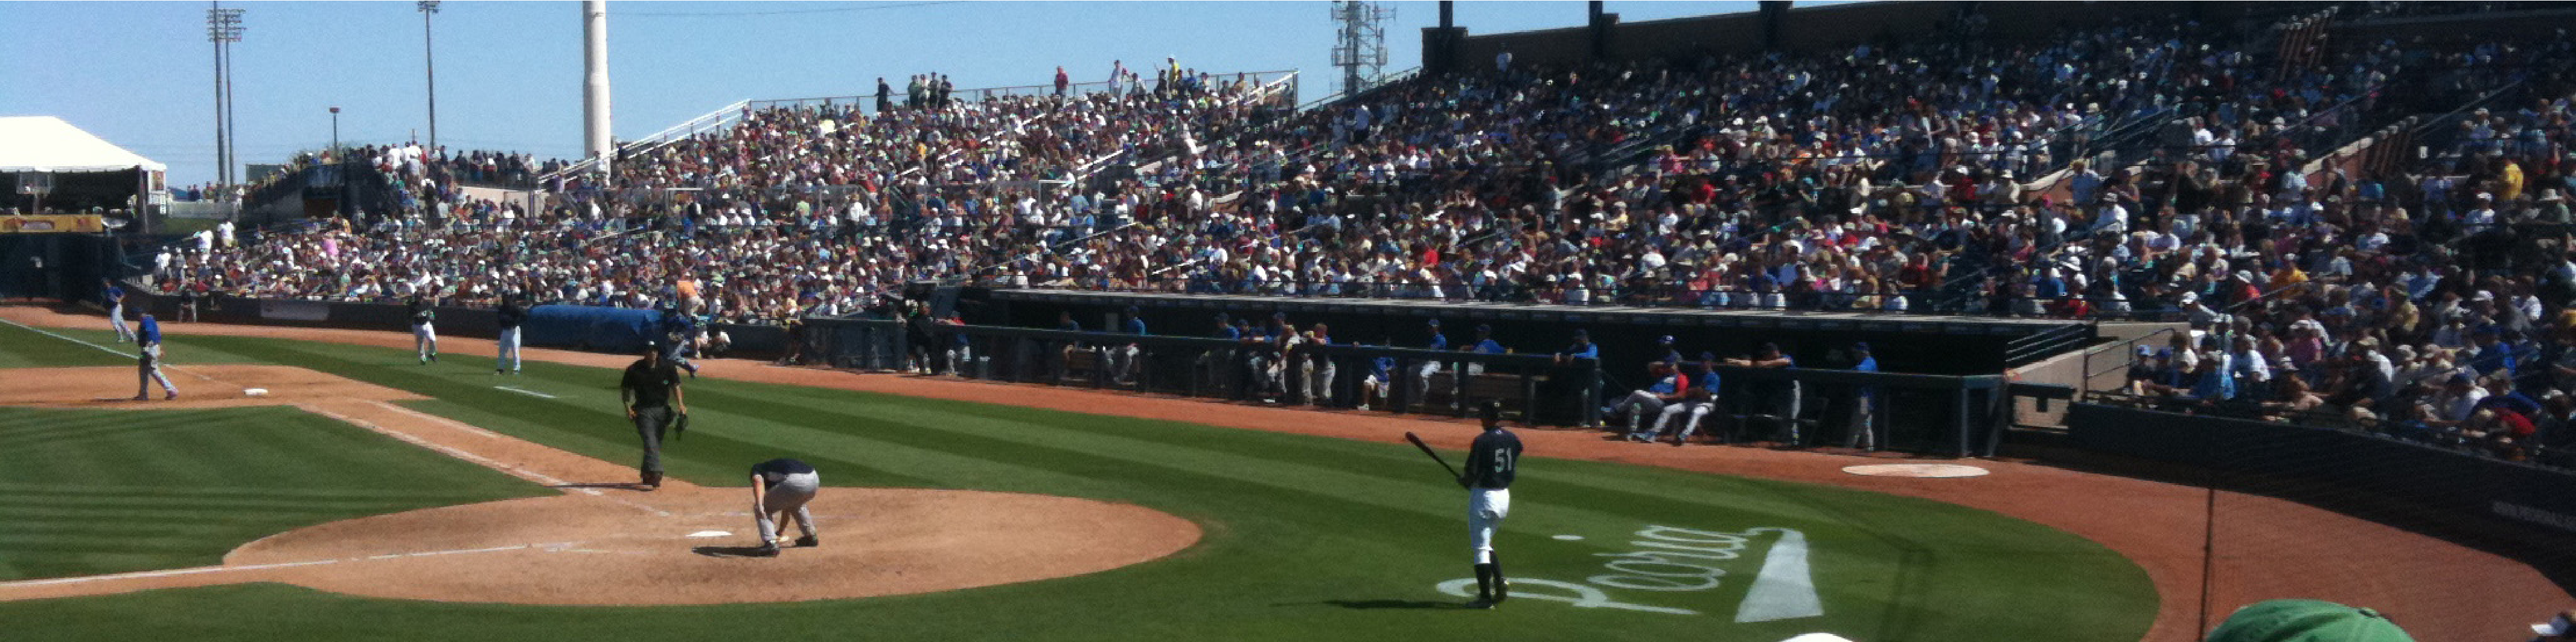
\includegraphics[height=1.5in]{images/sampleteaser}
%%   \caption{Spring Training 2009, Peoria, AZ.}
%% }

\maketitle

\begin{abstract}
	In this paper, we present a way to approximate real lighting for different time periods by using image based lighting with sparsely obtained light probes. In order to maintain 
	lighting consistency we use of interpolation, we have tested and compared a few interpolation methods.
\end{abstract}

\begin{CRcatlist}
  \CRcat{I.3.3}{Computer Graphics}{Three-Dimensional Graphics and Realism}{image based lighting}
  \CRcat{I.3.7}{Computer Graphics}{Three-Dimensional Graphics and Realism}{global illumination};
\end{CRcatlist}

\keywordlist

%% Use this only if you're preparing a technical paper to be published in the 
%% ACM 'Transactions on Graphics' journal.

\TOGlinkslist

%% Required for all content. 

\copyrightspace

\section{Introduction}

Computer graphics is present in a wide variety of areas ranging from entertainment to medicine or military applications, and one of its biggest challenges is generating realistic and 
convincing synthetic scenes. Realistic scene synthesis is dependent on a few factors, like geometry, materials and lighting. One of the most complex elements to reproduce are those 
related to lighting.

We would like to render scenes in different periods of the day with realistic and convincing lighting. Realistic lighting can be achieved by means of a technique called Image 
Based Lighting. Image Based Lighting (IBL) consists in obtaining light probes, which are omnidirectional High Dynamic Range images, and using them as environment maps during the rendering phase.

However, this technique is limited in the sense that we must obtain a new light probe for every instant we would like to render. This limitation makes the use of image-based lighting 
inviable depending on the time range of the scenes to be rendered due to enormous amount of work involved in obtaining the light probes.

Our main goal is to alleviate the restriction that a light probe must be obtained for every moment to be rendered. In order to do that we propose the use of interpolation to estimate 
the light probes for the instants that data is not available.

We propose two comparisons to validate our approximation:
\begin{itemize}
	\item Comparing light probes obtained through interpolation and light probes obtained through the usual way, which is done by combining different exposure time images.
	\item Comparing the rendering a simple object using the interpolated light probe as a light source and the same object in the real scene. The object is a white cube see Figure \ref{fig:whitecube}.
\end{itemize}

\begin{figure}[!ht]
	\caption{White cube used for comparison.}
	\centering
	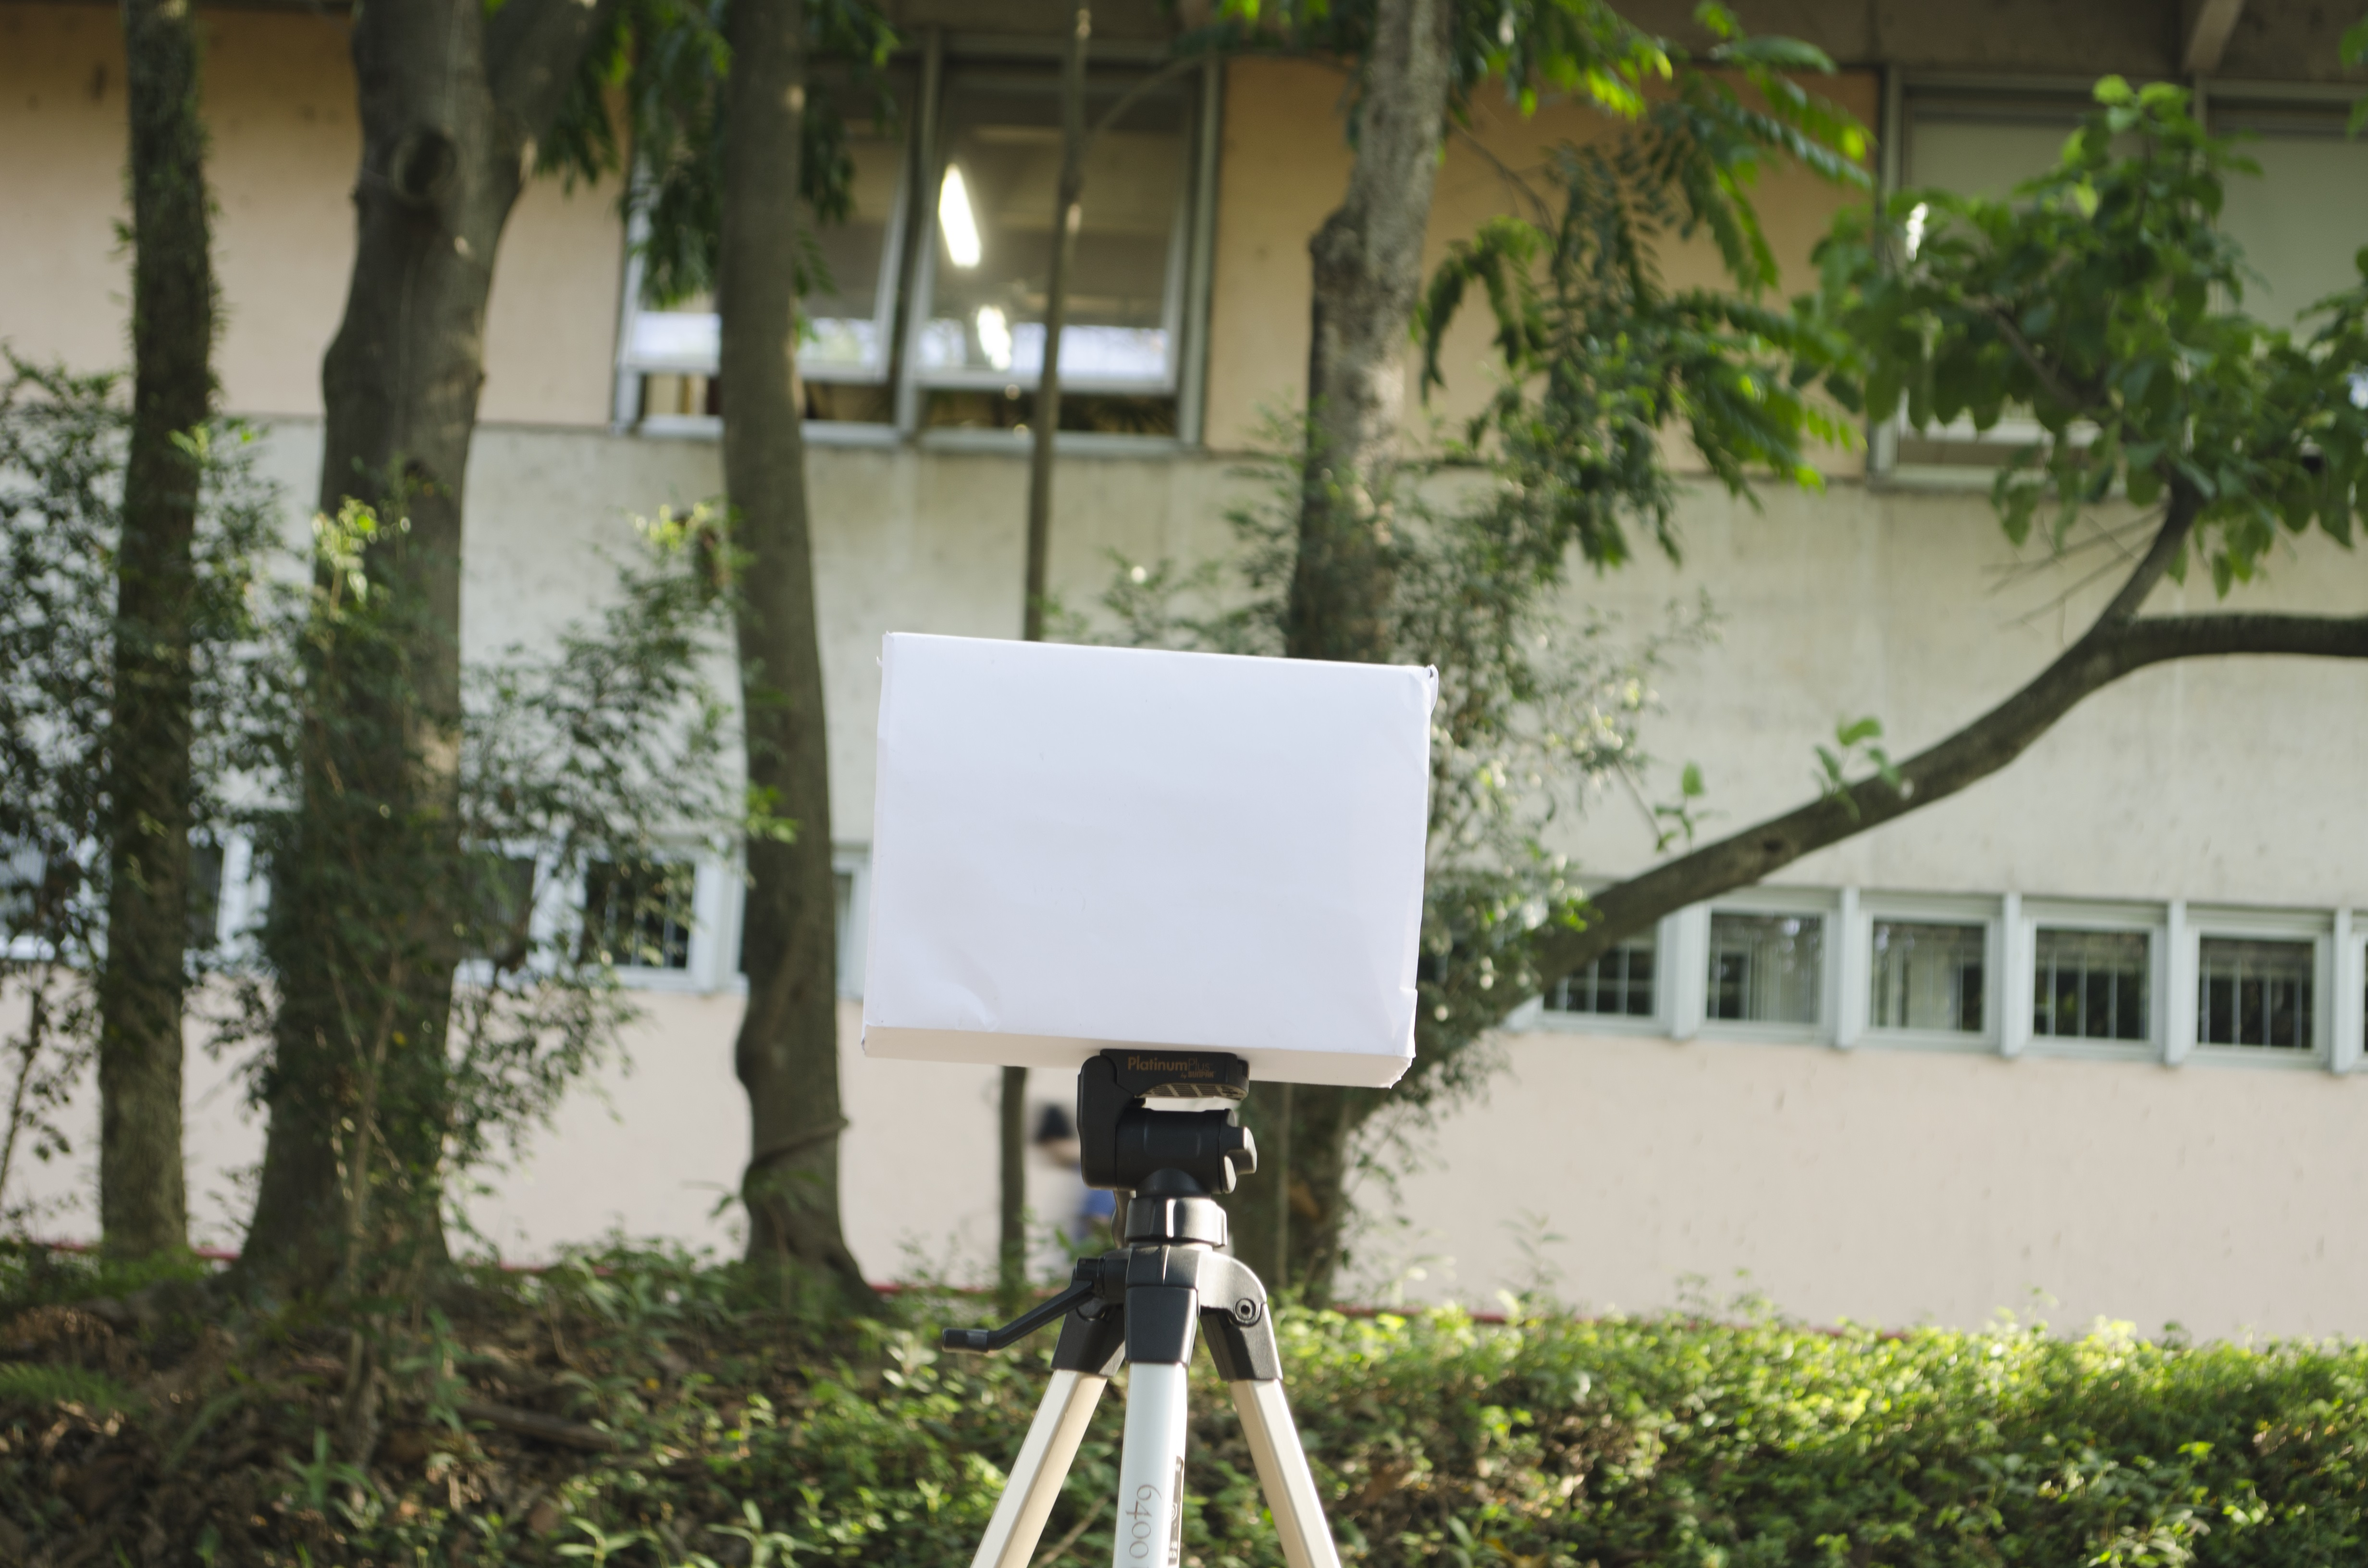
\includegraphics[width=8cm]{images/ext2.jpg}
	\label{fig:whitecube}
\end{figure}

\section{Definitions}

\subsection{Environment Map}

	Environment mapping \cite{hughes2013} consists in exchanging the illumination model for a texture lookup model which contains the lighting information.

\subsection{High Dynamic Range}

	High Dynamic Range (HDR) is an image format capable of representing a scene’s great variation in luminosity. It is usually stored using floating points with 32 bits per channel. 
	HDR images can be obtained by using special cameras like the Spheron \cite{spheron}, or combining images with different exposure times using software like Photoshop or HDR Shop. 
	A scene’s radiance can be recovered from a scene’s HDR image \cite{debevec1997}.

\subsection{Image Based Lighting}

	Image Based Lighting (IBL) \cite{debevec2002} consists in capturing a scene illumination information through an omnidirectional HDR image. To capture omnidirectional images either 
	a reflective sphere (Figure \ref{fig:lightprobe}\cite{linda2007}) or fisheye lenses (Figure \ref{fig:fisheye}\cite{salgado2010}) can be used. The resulting image, called light probe, is then used as an environment 
	map in the rendering phase. Note that a new light probe must be acquired for different locations or periods, otherwise the lighting consistency might not be maintained.

	\begin{figure}[!ht]
		\caption{Image obtained by using a fisheye lens.}
		\centering
		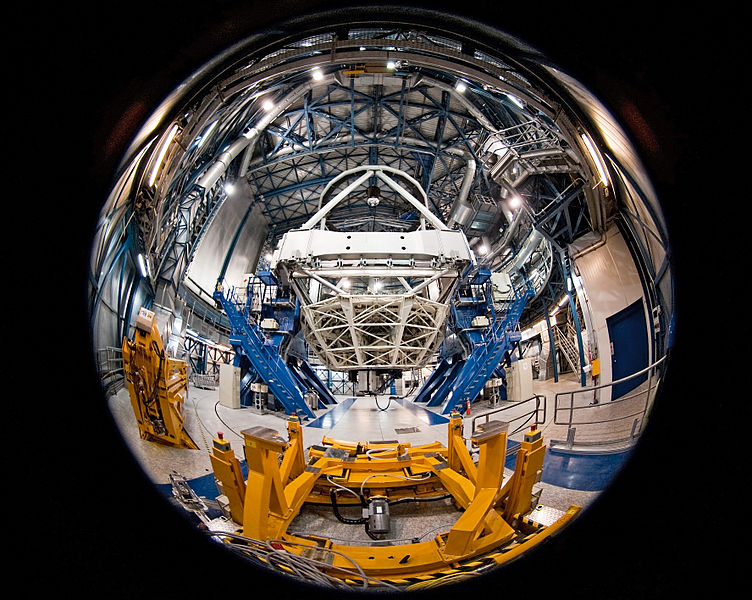
\includegraphics[width=6cm]{images/fisheye.jpg}
		\label{fig:fisheye}
	\end{figure}

	\begin{figure}[!ht]
		\caption{Reflective sphere that could be used as a light probe.}
		\centering
		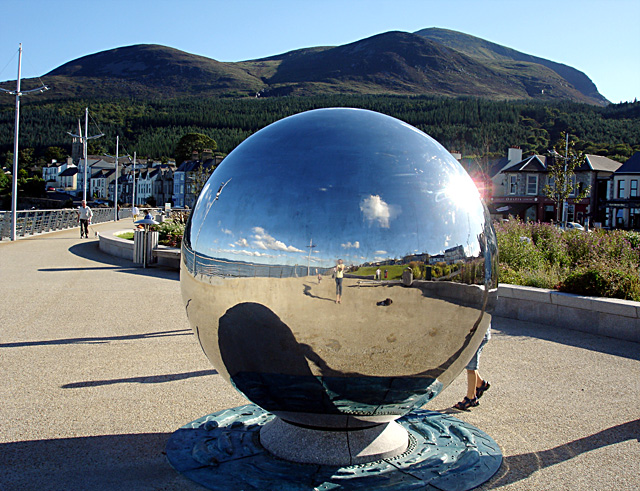
\includegraphics[width=6cm]{images/lightprobe.jpg}
		\label{fig:lightprobe}
	\end{figure}

\subsection{Interpolations}
	We have used five types of  interpolations to generate new light probes from our data. The light probes were interpolated  using pixel intensities over time.
For every interpolation method the set of light probes is represented by $(\dots,y_{i-2},y_{i-1},y_i,y_{i+1},y_{i+2},\dots)$, ordered by the time of acquisition.
The acquisition time, or observation, is represented by the set $(\dots,x_{i-2},x_{i-1},x_i,x_{i+1},x_{i+2},\dots)$, ordered in crescent manner. The interpolated
light probe is $y'$ in the formulae below.
\subsubsection{Linear Interpolation}
	The first interpolation is the classic linear interpolation. Its formula is as below: 
\begin{align}
	y' = y_0 + (y_1-y_0)*\frac{x-x_0}{x_1-x_0}
\end{align}
Where $y$ represents the intensities of each pixel while $x$ represents the time associated with the light probe's acquisition.

\subsubsection{Gauss Forward Central Difference}
	The second interpolation method is the Gauss Forward Central Difference. The Forward interpolation uses an iterative method that adds the $n$-esieme central 
difference\cite{abramowitz1972handbook} using the pyramidal construction represented by Figure \ref{fig:fowardcentral}. This method and the next requires
that the observation times are acquired at an regular time interval $h$. The interpolation formula is:
\begin{align}
\begin{split}
	y' &= 	y_i + P \delta_{1/2} + G_2 \delta_0^2 + G_3 \delta_{1/2}^3 + \dots\\
	P &= (x-x_i)/h \\
	G_{2n} &= \binom{P+n-1}{2n} \\
	G_{2n+1} &= \binom{P+n}{2n+1}
\end{split}
\end{align}

\begin{figure}[H]
	\caption{Reflective sphere that could be used as a light probe.}
	\centering
	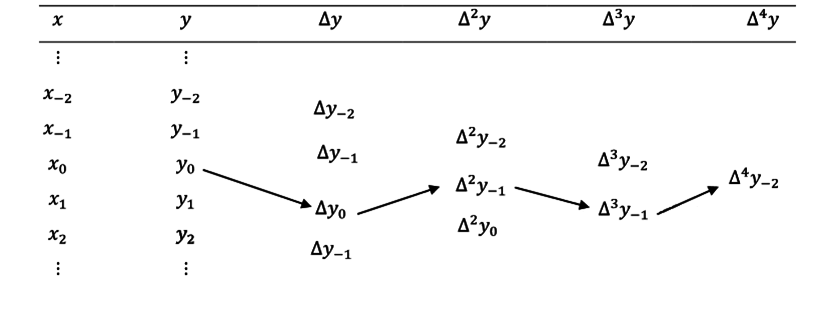
\includegraphics[width=08cm]{images/forward.png}
	\label{fig:fowardcentral}
\end{figure}

\subsubsection{Gauss Backward Central Difference}
	The Gauss Backward Central Difference diffesr from the Foward in the way that the iteraction chooses which central difference to use. 
It uses another direction in the pyramidal scheme to determine which central difference will be used. The selection algorithm is represented 
by Figure\ref{fig:backwardcentral}. The formula used is:
\begin{align}
\begin{split}
	y' &= y_i + P \delta_{-1/2} + G_2 \delta_0^2 + G_3 \delta_{-1/2}^3 + \dots\\
	P &= (x-x_i)/h \\
	G'_{2n} &= \binom{P+n}{2n} \\
	G_{2n+1} &= \binom{P+n}{2n+1}
\end{split}
\end{align}
	As stated above, the Backward interpolation 

\begin{figure}[H]
	\caption{Reflective sphere that could be used as a light probe.}
	\centering
	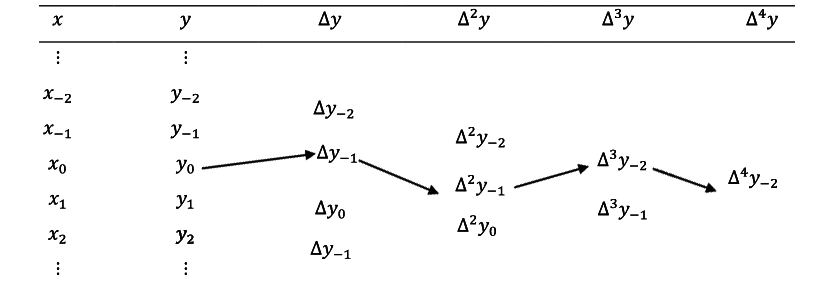
\includegraphics[width=08cm]{images/backward.png}
	\label{fig:backwardcentral}
\end{figure}

\subsubsection{Lagrange Interpolation}
	Lagrange’s interpolation advantage in relation to Gauss methods are that it does not require regularly spaced data to work, thus making the process of gathering the light probe images a little easier. The general formula for the Lagrange interpolation is:
\begin{align}
\begin{split}
	y' = \frac{(x-x_1)(x-x_2)\dots(x-x_n)}{(x_0-x_1)(x_0-x_2)\dots(x_0-x_n)}y_0 &+ \\
		 \frac{(x-x_0)(x-x_2)\dots(x-x_n)}{(x_1-x_0)(x_1-x_2)\dots(x_1-x_n)}y_1 &+ \\
		 \dots &\\
		 \frac{(x-x_0)(x-x_2)\dots(x-x_{n-1})}{(x_n-x_0)(x_n-x_2)\dots(x_n-x_{n-1})}y_n &
\end{split}
\end{align}

\subsubsection{Stirling's Interpolation}
	Stirling's interpolation can be calculated by taking the average of the Gauss Forward difference and the Gauss Backward difference. The formula
can be writen as:
\begin{align}
\begin{split}
	y' &= y_i + P \frac{\delta_{1/2}+\delta_{-1/2}}{2} + \\ &H_2 \delta_0^2 + H_3 \frac{\delta^3_{1/2}+\delta^3_{-1/2}}{2} + \dots\\
	P &= (x-x_i)/h \\
	H_{2n} &= \frac{G_2 + G'_2}{2} \\
	H_{2n+1} &= \binom{P+n}{2n+1}
\end{split}
\end{align}

\section{Experiment}
	As stated in the Introduction, we want to validate our interpolations by using two kinds of comparisons. In one of them, we compare interpolated light probes with the light probes obtained by conventional means, while in the other we compare a shot of a white cube with a rendering of a white cube, using image based lighting using an interpolated light probe that was created using the same time the shot was taken.

\subsection{Data Acquisition}
	To realize our experiments, we have acquired two sets of light probe data. The first set was taken outdoors, always in the same location, starting at 10:45 A.M. and ending 20:00 P.M. The second was acquired indoors, close to a window, commencing 11:00 A.M. and ending 19:45. We tried to take one shot every 30 minutes. For every shot, we also took a shot of a white cube. The Table \ref{tab:backwardcentral} 
\begin{center}
    \begin{tabular}{| l | l | l |}
	\hline
    \multicolumn{3}{|c|}{Data Acquisition Time} \\
    \hline
    \# & Outside & Inside \\
    \hline
    1 & 10:45 & 11:00 \\
    \hline
    2 & 11:20 & 11:30 \\
    \hline
    3 & 11:52 & 12:02 \\
    \hline
    4 & 12:18 & 12:30 \\
    \hline
    5 & 12:48 & 13:00 \\
    \hline
	6 & 13:18 & 13:30 \\
    \hline
	7 & 14:35 & 14:40 \\
    \hline
	8 & 15:05 & 15:10 \\
    \hline
    9 & 15:30 & 15:40 \\
    \hline
	10 & 16:00 & 16:10 \\
    \hline
	11 & 16:30 & 16:40 \\
    \hline
	12 & 17:05 & 17:15 \\
    \hline
	13 & 17:40 & 17:45 \\
    \hline
	14 & 18:05 & 18:15 \\
    \hline
	15 & 18:35 & 18:45 \\
    \hline
	16 & 19:05 & 19:15 \\
    \hline
	17 & 19:35 & 19:45 \\
    \hline
	18 & 20:00 & \\
    \hline
    \end{tabular}
    \label{tab:backwardcentral}
\end{center}

\subsection{Data Validation}

\subsection{Interpolated light probes}
	To create both the linear and Lagrange interpolated light probes we have used all data available with the real time associated with them. 
However, for the Gauss interpolated light probes we have used only a subset of the data available, the main reason for that was that we had to space our data evenly with at least a one-hour interval between them., For Gauss interpolation, we have considered that the time difference between each acquisition for the light probes 8 through 20 was 30 minutes.

\subsection{Distance between HDR images}
	We have defined a simple distance to compare two HDR images, which is given by:
\begin{align}
\begin{split}
	d = \sum\limits_{i}^{n} \sum\limits_{j}^{n} \sum\limits_{channel} \mid Image1[i][j].channel - Image2[i][j].channel \mid
\end{split}
\end{align}

\subsubsection{Rendering the White Cube}
	Using the distance previously defined, we have determined for each of the chosen scenes two interpolations with least distance compared to the real light probe. These interpolations were used to render a white cube modeled in Maya. The chosen renderer was nvidia’s Mental Ray, which supports image based lighting.

\section{Results}

\section{Conclusion}

\section*{Acknowledgements}

\bibliographystyle{acmsiggraph}
\bibliography{template}
\end{document}
